\subsubsection{Syntax Trees}


Now that the parser for the given file has been generated by gt it is ready to be used. 
Figure 2.3 shows the syntax tree that is generated by the above grammar.
%
%
%
\begin{figure}[h!]
  \centering
  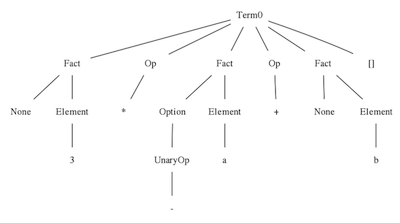
\includegraphics[width=4in]{./examples/ebnf/arith/ebnf-arith.png}
  \caption{Syntax Tree for\\ \textit{3 * -a + b}}
\end{figure}